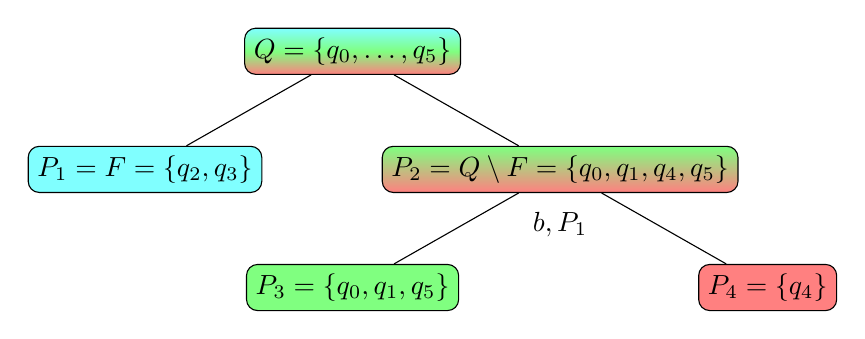
\begin{tikzpicture}[sibling distance=15em, every node/.style = {shape=rectangle, rounded corners, draw, align=center}]
	\node[top color=cyan!50, bottom color=red!50, middle color=green!50] {$Q = \{q_0, \ldots, q_5\}$}
		child { node[top color=cyan!50, bottom color=cyan!50] {$P_1 = F = \{q_2, q_3\}$} }
		child { node[top color=green!50, bottom color=red!50]  {$P_2 = Q \setminus F = \{q_0, q_1, q_4, q_5\}$} 			
			child { node[top color=green!50, bottom color=green!50] {$P_3 = \{q_0, q_1, q_5\}$} }
			child { node[top color=red!50, bottom color=red!50] {$P_4 = \{q_4\}$} }
			node[draw=none, yshift=-20pt] {$b, P_1$} };
\end{tikzpicture}